\chapter{OSTES Validation}
\label{chap:OSTESValid}

The OSTES algorithm was tested on synthetic data and on data acquired with the ASTER sensor. The results show that the OSTES algorithm improves temperature and emissivity retrievals in several ways. The most significant improvement occurs for surfaces with low spectral contrast, which is one of the major weaknesses of the original version of TES algorithm. The temperature and emissivity estimations from OSTES are more accurate in these cases. The investigation of OSTES with simulated data also shows that the algorithm is less sensitive to seasonal fluctuations in atmospheric and surface temperature.

\section{Imaging Systems}

From the wide range of airborne sensors operating in the TIR region two are chosen as examples: Airborne Hyperspectral Scanner (AHS) operated by Spanish Institute of Aeronauics (INTA) and developed by ArgonST (Fairfax, USA), and Thermal Airborne Spectrographic Imager (TASI) developed by Itres Ltd. (Calgary, Canada). These sensors offer data of great importance in applications. Notable studies include areas of
mineral mapping \cite{NK14}, 
soil moisture estimation \cite{SF12}, 
urban studies \cite{SO12},
soil organic carbon estimation \cite{PC14} and
crop water stress characterization \cite{PP12},
among others.

\begin{figure}[!t]
	\centering
	\vspace{1em}
	\begin{subfigure}[t]{\linewidth}
		\centering
		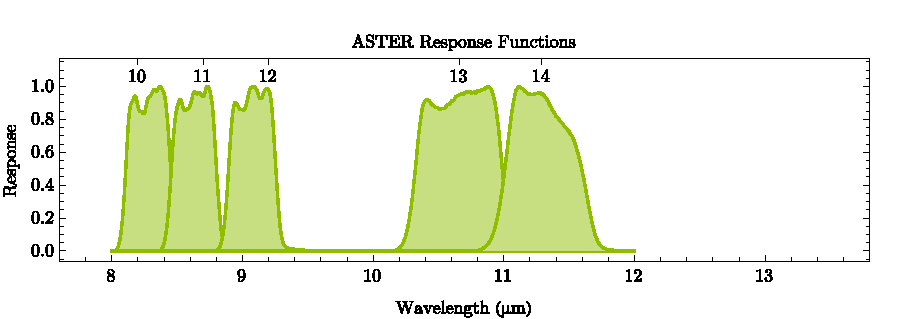
\includegraphics[scale=1]{pics/Chapter_04/Response_functions_ASTER-eps-converted-to.pdf}
		\caption{}
		\vspace{0.5em}
	\end{subfigure}
	\hspace{1em}
	\begin{subfigure}[t]{\linewidth}
		\centering
		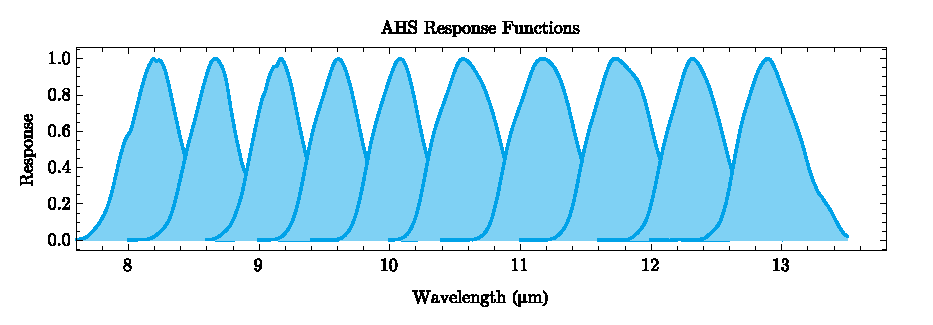
\includegraphics[scale=1]{pics/Chapter_04/Response_functions_AHS.eps}
		\caption{}
		\vspace{0.5em}
	\end{subfigure}
	\hspace{1em}
	\begin{subfigure}[t]{\linewidth}
		\centering
		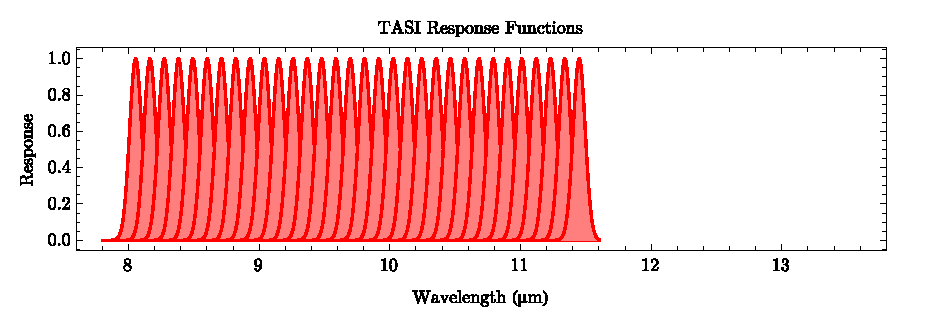
\includegraphics[scale=1]{pics/Chapter_04/Response_functions_TASI.eps}
		\caption{}
	\end{subfigure}
	\vspace{1 em}
	\caption{Response functions for (a) ASTER, (b) AHS  and (c) TASI sensors. The ASTER Band Numbers are shown above the ASTER response functions. }
	\label{fig:emissivitySpectra_spectra}
\end{figure}

The above-mentioned airborne sensors were chosen together with the ASTER sensor to analyze the performance of the OSTES algorithm.
%\subsubsection{ASTER}
ASTER consists of 15 bands of which 5 are situated in TIR region with Noise Equivalent Temperature difference $\mathrm{(NE\Delta T)} \approx 0.3\,\mathrm{K}$. The spatial resolution of the TIR bands is $90\,\mathrm{m}$.
%\subsubsection{AHS}
The AHS sensor has been fully operational from 2005 \cite{FM05}. Its sensor operates in 80 spectral bands where the last 10 bands cover atmospheric window from 8 to $13\,\mathrm{\mu m}$ \cite{SJ06}. The AHS TIR bands have a  {Full Width at Half Maximum} $\mathrm{(FWHM)} \approx 0.5\,\mathrm{\mu m}$ with $\mathrm{NE\Delta T} \approx 0.5\,\mathrm{K}$.
%\subsubsection{TASI}
 {The third sensor we will consider is TASI sensor,} one of the very few commercially available hyperspectral TIR sensors. It contains 32 bands all of which are in the TIR region. Bands are situated in the 8 to $11.5\,\mathrm{\mu m}$ region and have a $\mathrm{FWHM} \approx 0.11\,\mathrm{\mu m}$ with $\mathrm{NE\Delta T} \approx 0.1\,\mathrm{K}$. The response functions of these sensors are depicted in Fig. \ref{fig:ResponseFunctions}.

\begin{table}[thb]
\vspace{0.5em}
\footnotesize
\centering
\begin{tabular}{lcccc}
\toprule
Sensor & $a$ & $b$ & $c$ & $r^2$\\ \hline
ASTER & $0.994$ & $-0.687$ & $0.737$ & $0.983$ \\
AHS & $1.000$ & $-0.782$ & $0.817$ & $0.994$ \\
TASI & $1.001$ & $-0.737$ & $0.760$ & $0.997$ \\
\bottomrule
\end{tabular}
\vspace{1.5 em}
\caption{Regression coefficients of $\varepsilon_\mathrm{min} = a + b\:\mathrm{MMD}^c$ and coefficients of determination $r^2$}
\label{table:MMDcoef}
\normalsize
\end{table}

\section{Simulated Data}

A data set of 6588 samples was artificially created to compare the performance of the TES and OSTES algorithms. Samples include 108 different natural surfaces chosen from ASTER spectral library \cite{BH09} at different temperatures coupled with 61 different atmospheric conditions taken from TIGR (TOVS Initial Guess Retrieval) database \cite{CS85, CC98}. 
These samples were processed to land-leaving and downwelling radiance, as standard TES algorithm input, and they were transformed to band-effective quantities with respect to the ASTER, AHS and TASI response functions.

\begin{figure}[!t]
	\centering
	\vspace{1em}
	\begin{subfigure}[t]{.3\linewidth}
		\centering
		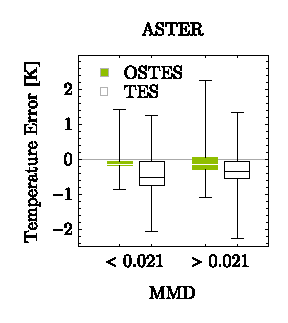
\includegraphics[scale=1]{pics/Chapter_04/Simulated_data_ASTER.eps}
		\caption{}
	\end{subfigure}
	\hspace{1em}
	\begin{subfigure}[t]{.3\linewidth}
		\centering
		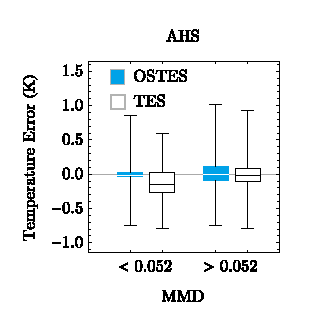
\includegraphics[scale=1]{pics/Chapter_04/Simulated_data_AHS.eps}
		\caption{}
	\end{subfigure}
	\hspace{1em}
	\begin{subfigure}[t]{.3\linewidth}
		\centering
		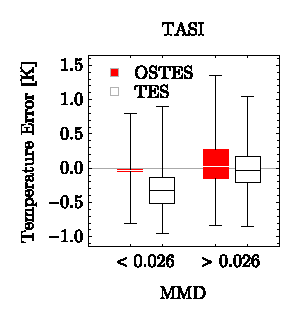
\includegraphics[scale=1]{pics/Chapter_04/Simulated_data_TASI.eps}
		\caption{}
	\end{subfigure}
	\vspace{1.5 em}
	\caption{Emissivity spectra (black solid line) of three samples chosen from ASTER spectral library \cite{BH09}. Symbols represent band-effective values of emissivity (empty symbols) and brightness temperature (full symbols) for ASTER (orange triangles), AHS (blue squares), and TASI (green dots) sensor. }
	\label{fig:ResponseFunctions}
\end{figure}

Simulated data for the ASTER sensor were processed with current implementation with revisions as described in \cite{GG06} and \cite{SG09}. We were, however, successful in getting our simulated data processed with the operational TES code. of TES, as it is used for generation of ASTER standard products AST\_05 and AST\_08 \cite{B15}. The version of the original TES algorithm in cases of AHS and TASI sensors was implemented in a manner similar to that described in \cite{JS12}. In addition, the implementation omits the $\varepsilon_\mathrm{max}$ refinement for emissivities with low spectral contrast. The OSTES was applied to all sensors as it is described in previous section.

\begin{table}[thb]
\vspace{0.5em}
\footnotesize
\centering
\begin{tabular}{cccc}
\toprule
Sensor & MMD & OSTES & TES \\ \hline
ASTER 	& $< 0.021$ & 0.25 & 0.50 \\
 		& $> 0.021$ & 0.36 & 0.43 \\ \hline
AHS 		& $< 0.052$ & 0.13 & 0.20 \\
 		& $> 0.052$ & 0.20 & 0.19 \\ \hline
TASI 	& $< 0.026$ & 0.16 & 0.32 \\
 		& $> 0.026$ & 0.32 & 0.30 \\
\bottomrule
\end{tabular}
\vspace{1.5 em}
\caption{Standard deviations of temperature errors obtained by applying OSTES and TES algorithm on simulated data as seen by ASTER, AHS and TASI grouped according to the sample Maximum-Minimum emissivity Difference (MMD). }
\label{table:StandardDeviations}
\normalsize
\end{table}

Samples were passed to the TES and OSTES algorithms and the temperature and emissivity results were compared with true values. We divide the results into two groups according to the emissivity spectral contrast. For each sensor type we determined a threshold for Maximum-Minimum emissivity Difference (MMD) in order to separate the samples with small spectral contrast such as water, vegetation, snow or samples with small particle sizes from other samples with higher spectral contrast. The threshold was determined for each sensor separately since different response functions and spectral ranges result in different MMD values for the same sample. The performance of both TES versions was determined by subtracting retrieved temperature from true temperature value. The temperature error and chosen MMD values for ASTER, AHS and TASI are shown in Fig. \ref{fig:SimualtedDataTemperatureErrorVsLowVsHighMMD}.

It can be seen that temperature and emissivity retrieved with OSTES are more accurate for samples with low spectral contrast. On the other hand, no significant improvement is evident in cases of samples with higher spectral contrast. 

Let us remind the reader that every sample is processed under several different atmospheric conditions coupled with different sample temperatures. Thus the standard deviation of temperature and emissivity error is indicative of the algorithm’s sensitivity to seasonal fluctuations. A comparison of standard deviations of temperature errors introduced by both TES approaches reveals that the OSTES is less sensitive to changes in atmosphere and sample temperature for samples with low MMD. However, the standard deviations of temperature errors of samples with higher MMD are similar. Standard deviations of temperature errors obtained by the OSTES and TES algorithms are summarized in the Table \ref{table:StandardDeviations}.

\begin{figure*}[!t]
\centering
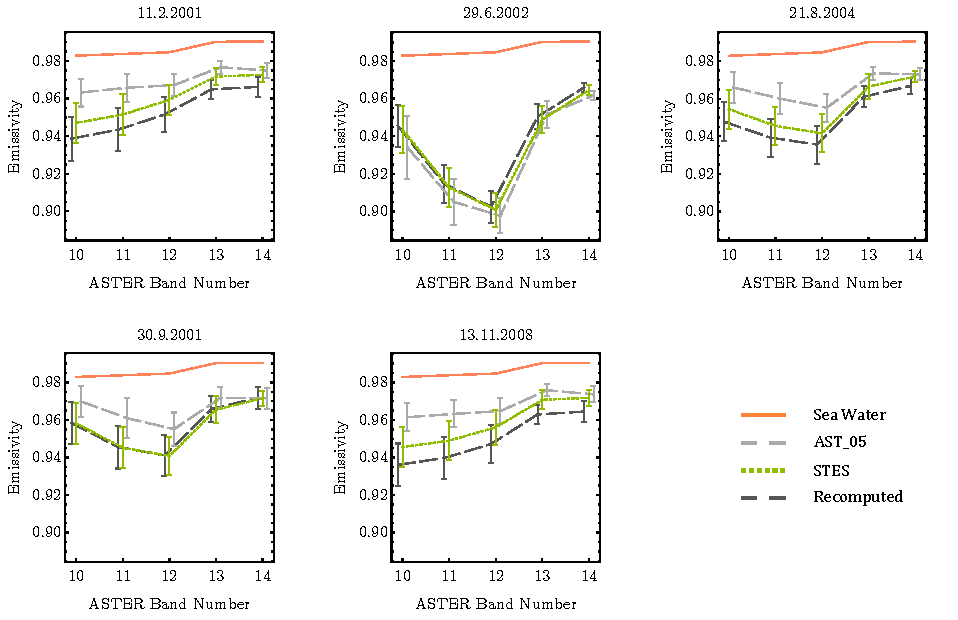
\includegraphics[width=0.95\linewidth]{pics/Chapter_04/Caspian.pdf}
\vspace{1.5 em}
\caption{Emissivity of Caspian Sea in different seasons obtained from ASTER standard product AST\_05, OSTES retrieval, and emissivity recomputation according to the temperature from AST\_08 and land-leaving and downwelling radiance from AST\_09T. Emissivities were extracted from area of size $40 \times 40$ pixels over pure and cloudless waterbody. Error bars display standard deviation.}
\label{fig:CaspianSeaEmissivity}
\end{figure*}

\section{Comparison with ASTER standard products}

The performance of the OSTES algortihm was also tested and compared with standard ASTER products. Testing is focused on: 1) investigating the impact of seasonal changes on emissivity retrievals, and 2) emissivity smoothness over homogeneous areas. Both tasks were performed on ASTER scenes containing large water bodies. For the first task we chose five scenes of the Caspian Sea acquired in various seasons of the year. For the second task we chose Lake Baikal. The list of all scenes used, together with their acquisition and processing date is given in Table \ref{table:ASTERScenes}. For every scene we downloaded ASTER standard products AST\_09T, AST\_08 and AST\_05 delivering land-leaving and downwelling radianace, surface kinetic temperature and surface emissivity, respectively. Product AST\_09T was used as input to the OSTES algorithm. The resulting temperature and emissivity was then compared with the AST\_08 and AST\_05 standard products. The emissivity variability over large and homogeneous area was chosen to be the quality indicator, since we are interested in the retrieval of material properties, which should be constant within the time and space.

\begin{table}[thb]
\vspace{0.5em}
\footnotesize
\centering
\begin{tabular}{ccc}
\toprule
Location & Acq date & Processing date \\ \hline
% &  &  \\
Caspian Sea & 11.02.2001 - 07:35:55 (UTC) & 19.11.2015 \\
Caspian Sea & 30.09.2001 - 07:35:57 (UTC) & 19.11.2015 \\
Caspian Sea & 29.06.2002 - 07:31:47 (UTC) & 19.11.2015 \\
Caspian Sea & 21.08.2004 - 07:29:35 (UTC) & 19.11.2015 \\
Caspian Sea & 13.11.2008 - 07:24:21 (UTC) & 19.11.2015 \\
Lake Baikal & 22.07.2002 - 04:17:29 (UTC) & 27.08.2015 \\
\bottomrule
\end{tabular}
\vspace{1.5 em}
\caption{ASTER scenes used for algorithm testing}
\label{table:ASTERScenes}
\normalsize
\end{table}

From the Caspian Sea scenes we chose samples of size $40 \times 40$ pixels over uniform, cloudless waterbody. These subsets were processed by the OSTES algorithm and the emissivity results were averaged for every scene. The results are plotted in Fig. \ref{fig:CaspianSeaEmissivity} along with the emissivities that were delivered in the AST\_05 product and averaged over the same spatial subset. In most cases the AST\_05 emissivity spectra appear to be closer to the sea water emissivity spectra taken from ASTER spectral library \cite{BH09}. However, the temperature retrievals of extracted samples obtained by OSTES and TES are very close (not shown). The average temperature difference of AST\_08 and OSTES results computed from all Caspian Sea samples is 0.2\,K (s.d. 0.2\,K). The fact that the temperatures obtained with the two algorithms are very close, but the emissivities are not implies that the emissivity spectra from AST\_05 product are not consistent with temperature from AST\_08 product. We verified this inconsistency by taking the temperatures delivered in AST\_08 and the downwellig and land-leaving radiances delivered in AST\_09T and putting these into (\ref{eq:emissivityComputation}) to obtain emissivities that are different from what is in the AST\_05 product. These emissivity spectra derived from AST\_08 and AST\_09T, which we refer to as ``recomputed emissivities'', are depicted on Fig. \ref{fig:CaspianSeaEmissivity} as well. Comparing recomputed emissivity spectra and OSTES results shows that in scenes acquired on 29.6.2002 and 30.9.2001 are results similar. On the other hand OSTES results perform slightly better in scenes acquired on 11.2.2001, 21.8.2004 and 13.11.2008. Nevertheless, none of the emissivity spectra agrees with expected values.

The difference in emissivity obtained by the two versions of TES is further illustrated in the scene over Lake Baikal shown in Fig. \ref{fig:Bajkal}. In this figure the white squares on the images define a water body sample of size $90 \times 90$ pixels that was used to produce the values in the histograms below the images. The expected values of sea water emissivity (red vertical line) are included in the Fig. \ref{fig:Bajkal}. The histograms show the OSTES emissivity retrievals compared against the AST\_05 standard product, as well as the emissivity recomputed with respect to the temperature delivered by AST\_08 and land-leaving and downwelling radiance delivered by AST\_09T, as described in the previous paragraph. Inspection of the ASTER standard product AST\_05 shows step discontinuities in bands 10, 11 and 12 over the study sample, which is reflected in the bimodal distributions in the histograms and the noisy patterns in the left image. On the contrary, OSTES emissivity results are smoother and the histograms do not show any significant discontinuities. The recomputed and OSTES emissivity retrievals are similar. However, the OSTES emissivities tend to be closer to the expected values. In addition to the noise, striping is also visible in the image. This not consequence of the TES algorithm and is more deeply discussed in \cite{GA11}. Even though the AST\_05 and OSTES emissivities differ significantly in some bands, the temperature retrievals are very similar. The average difference is 0.25 K (s.d. 0.18 K). Similar to the discussion regarding Caspian Sea emissivity retrievals, it can also be concluded in this case that none of the emissivity spectra have satisfying values.

\begin{figure*}[!t]
\centering
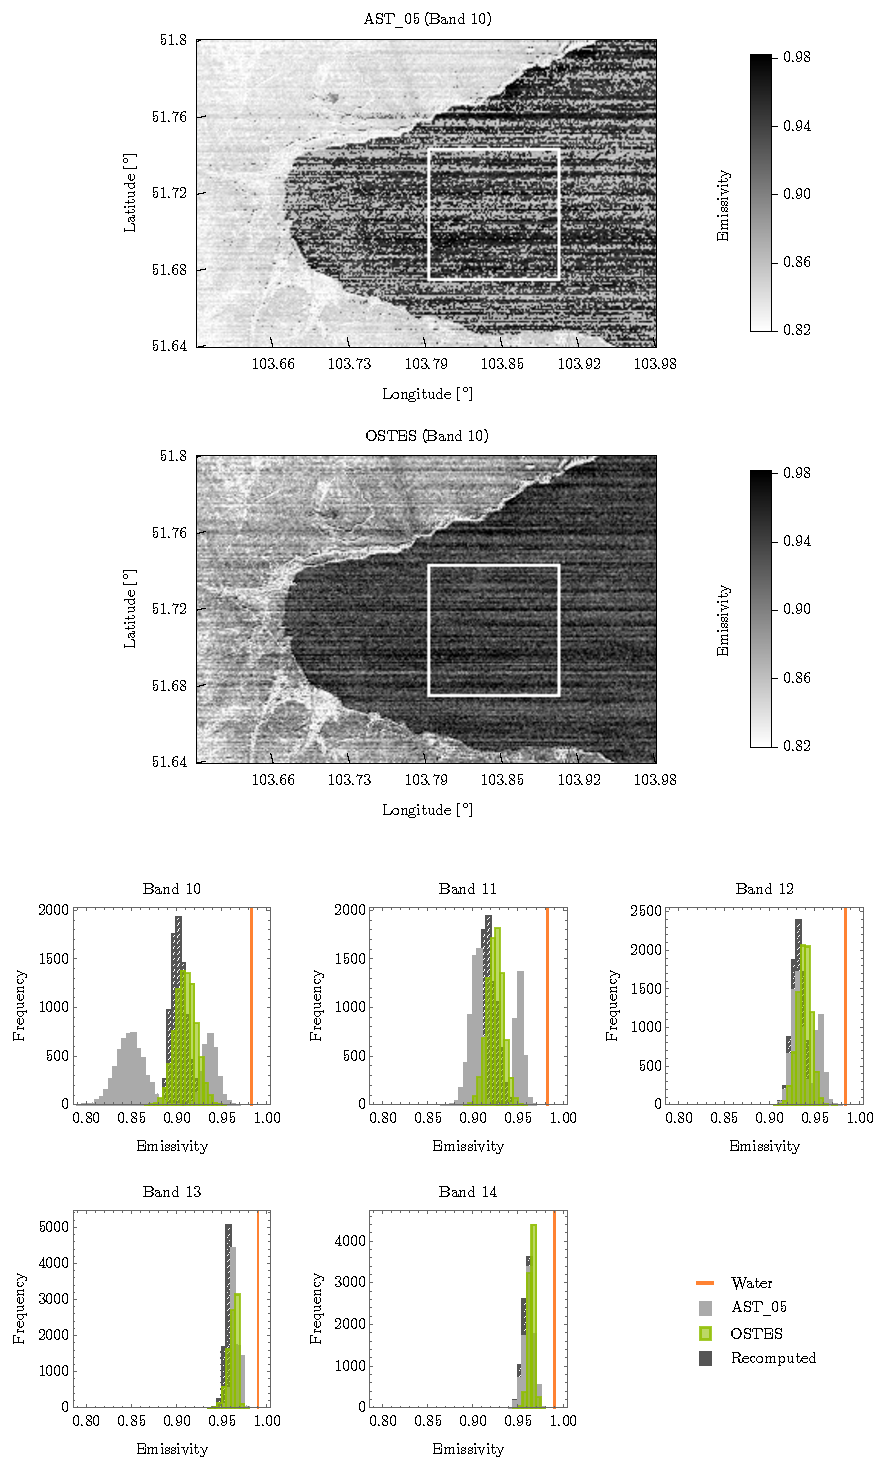
\includegraphics[width=0.78\linewidth]{pics/Chapter_04/Baikal.pdf}
\vspace{1.5 em}
\caption{
ASTER band 10 emissivity images of Lake Baikal obtained from ASTER standard product AST\_05 (upper left) and OSTES emissivity retrieval (upper right). In both images the same contrast stretching is used. The white square represents the area from which emissivity histrograms were created (lower panel). Histograms show distributions of AST\_05 emissivity, OSTES emissivity and recomputed emissivity according to the temperature from AST\_08 and land-leaving and downwelling radiance from AST\_09T. Line depicted in histograms indicates the expected value of water emissivity retrieved from ASTER spectral library \cite{BH09}.}
\label{fig:Bajkal}
\end{figure*}

The discrapancies in shape and magnitude of emissivity spectra can be caused by various source of errors but the main error source has been attributed to imperfect atmospheric corrections. The impact of this error is evident mainly in cases of low spectral constast. Notable works discussing emissivity retrievals with low spectral contrast are \cite{TP01, TP05, TP05-2, CC07, SJ07}. One suggested improvement is the water vapour scaling method \cite{T05, GA11}.

The step discontinuities in emissivity values over homogeneous area can occur due to various thresholds deciding how to treat the sample during processing. The original TES algorithm starts in the NEM module assuming a maximum emissivity spectra $\varepsilon_\mathrm{max}=0.99$. The NEM module is then restarted with refined $\varepsilon_\mathrm{max}$ according to the emissivity retrieved from the first NEM pass. Also,	 temperature and emissivity from NEM are reported as the result of TES algorithm if the correction for downwelling radiance is not possible. The original version of TES processes samples according to the MMD of emissivity spectra obtained from NEM module either by incorporating (\ref{eq:MMD}) or by presetting emissivity to $\varepsilon = 0.983$. Some authors \cite{GG06}, \cite{SG09} have suggested that the value of the threshold used for classifying observations into groups with either low or high spectral contrast should be changed or completely removed. Observations with wrongly determined spectral contrast or observations with spectral contrast close to any threshold result in step discontinuities. On the contrary, the OSTES does not set any thresholds for materials with low spectral contrast and so it is expected to generate smoother results on homogeneous areas with low spectral contrast.

\section{Application to TASI Data}

The study was performed using data acquired over the city of Brno, Czech Republic (49°12′N 16°37′E). The data examined come subset of one flight line crossing the city from south-west to north-east. The acquisition was performed on 4th July 2015 at 14:03 (UTC). The FLIS operated by Global Change Research Institute CAS (Brno, Czech Republic) \cite{HF14} was used for this acquisition. FLIS consists of Compact Airborne Spectrographic Imager (CASI), Shortwave infrared Airborne Spectrographic Imager (SASI) and Thermal Airborne Spectrographic Imager (TASI). All sensors are developed by Itres Ltd. (Calgary, Canada). In-situ emissivity measurements of urban materials were performed with FT-IR Spectrometer Models 102 developed by D\&P Instruments (Simsbury, USA). Emissivity spectra of water and deciduous trees were extracted from ASTER spectral library \cite{BH09}.

Data acquired by CASI, SASI and TASI sensor were radiometrically and atmospherically corrected and georeferenced to UTM coordinate system. Radiometric corrections were performed according to laboratory and in-flight sensor calibrations. Atmospheric corrections of TASI sensor are based on results of MODTRAN \cite{BG06}. Atmospheric temperature and water vapor profiles, as inputs to MODTRAN, were obtained from MODIS product MOD07\_L2.

The comparison of  the TES and the OSTES algorithms performance was tested against six \textit{in-situ} measurements of different urban surfaces. Results are shown in Fig. \ref{fig:BrnoEmissivityComparison} below, where error bars display standard deviation. The OSTES performs slightly better than TES in cases of deciduous trees and Svratka river. However, none of these two spectra agrees with the shape and magnitude of expected emissivity spectra. These discrepancies can be caused by various sources of errors but the main error source has been attributed to imperfect atmospheric corrections. Emissivities of sample 5 (Asphalt Parking Lots) retrieved by the TES and OSTES significantly differs from \textit{in-situ} measurement. This shift in magnitude is introduced by insufficient compensation of downwelling radiance. This sample is surrounded by buildings, which increase the amount of downwelling radiance. This additional radiance is not included in temperature and atmospheric profiles obtained from MOD07\_L2. The rest of the emissivity retrievals are considered to follow \textit{in-situ} measurements well. Let us emphasize the reader that OSTES offers only moderate improvements in emissivity retrievals. These are not possible to observe in this study due to the magnitude of error introduced by imperfect atmospheric corrections. We conclude that improvement of atmospheric corrections are crucial for further analysis.

\begin{figure*}[!t]
\centering
\vspace{0.8 em}
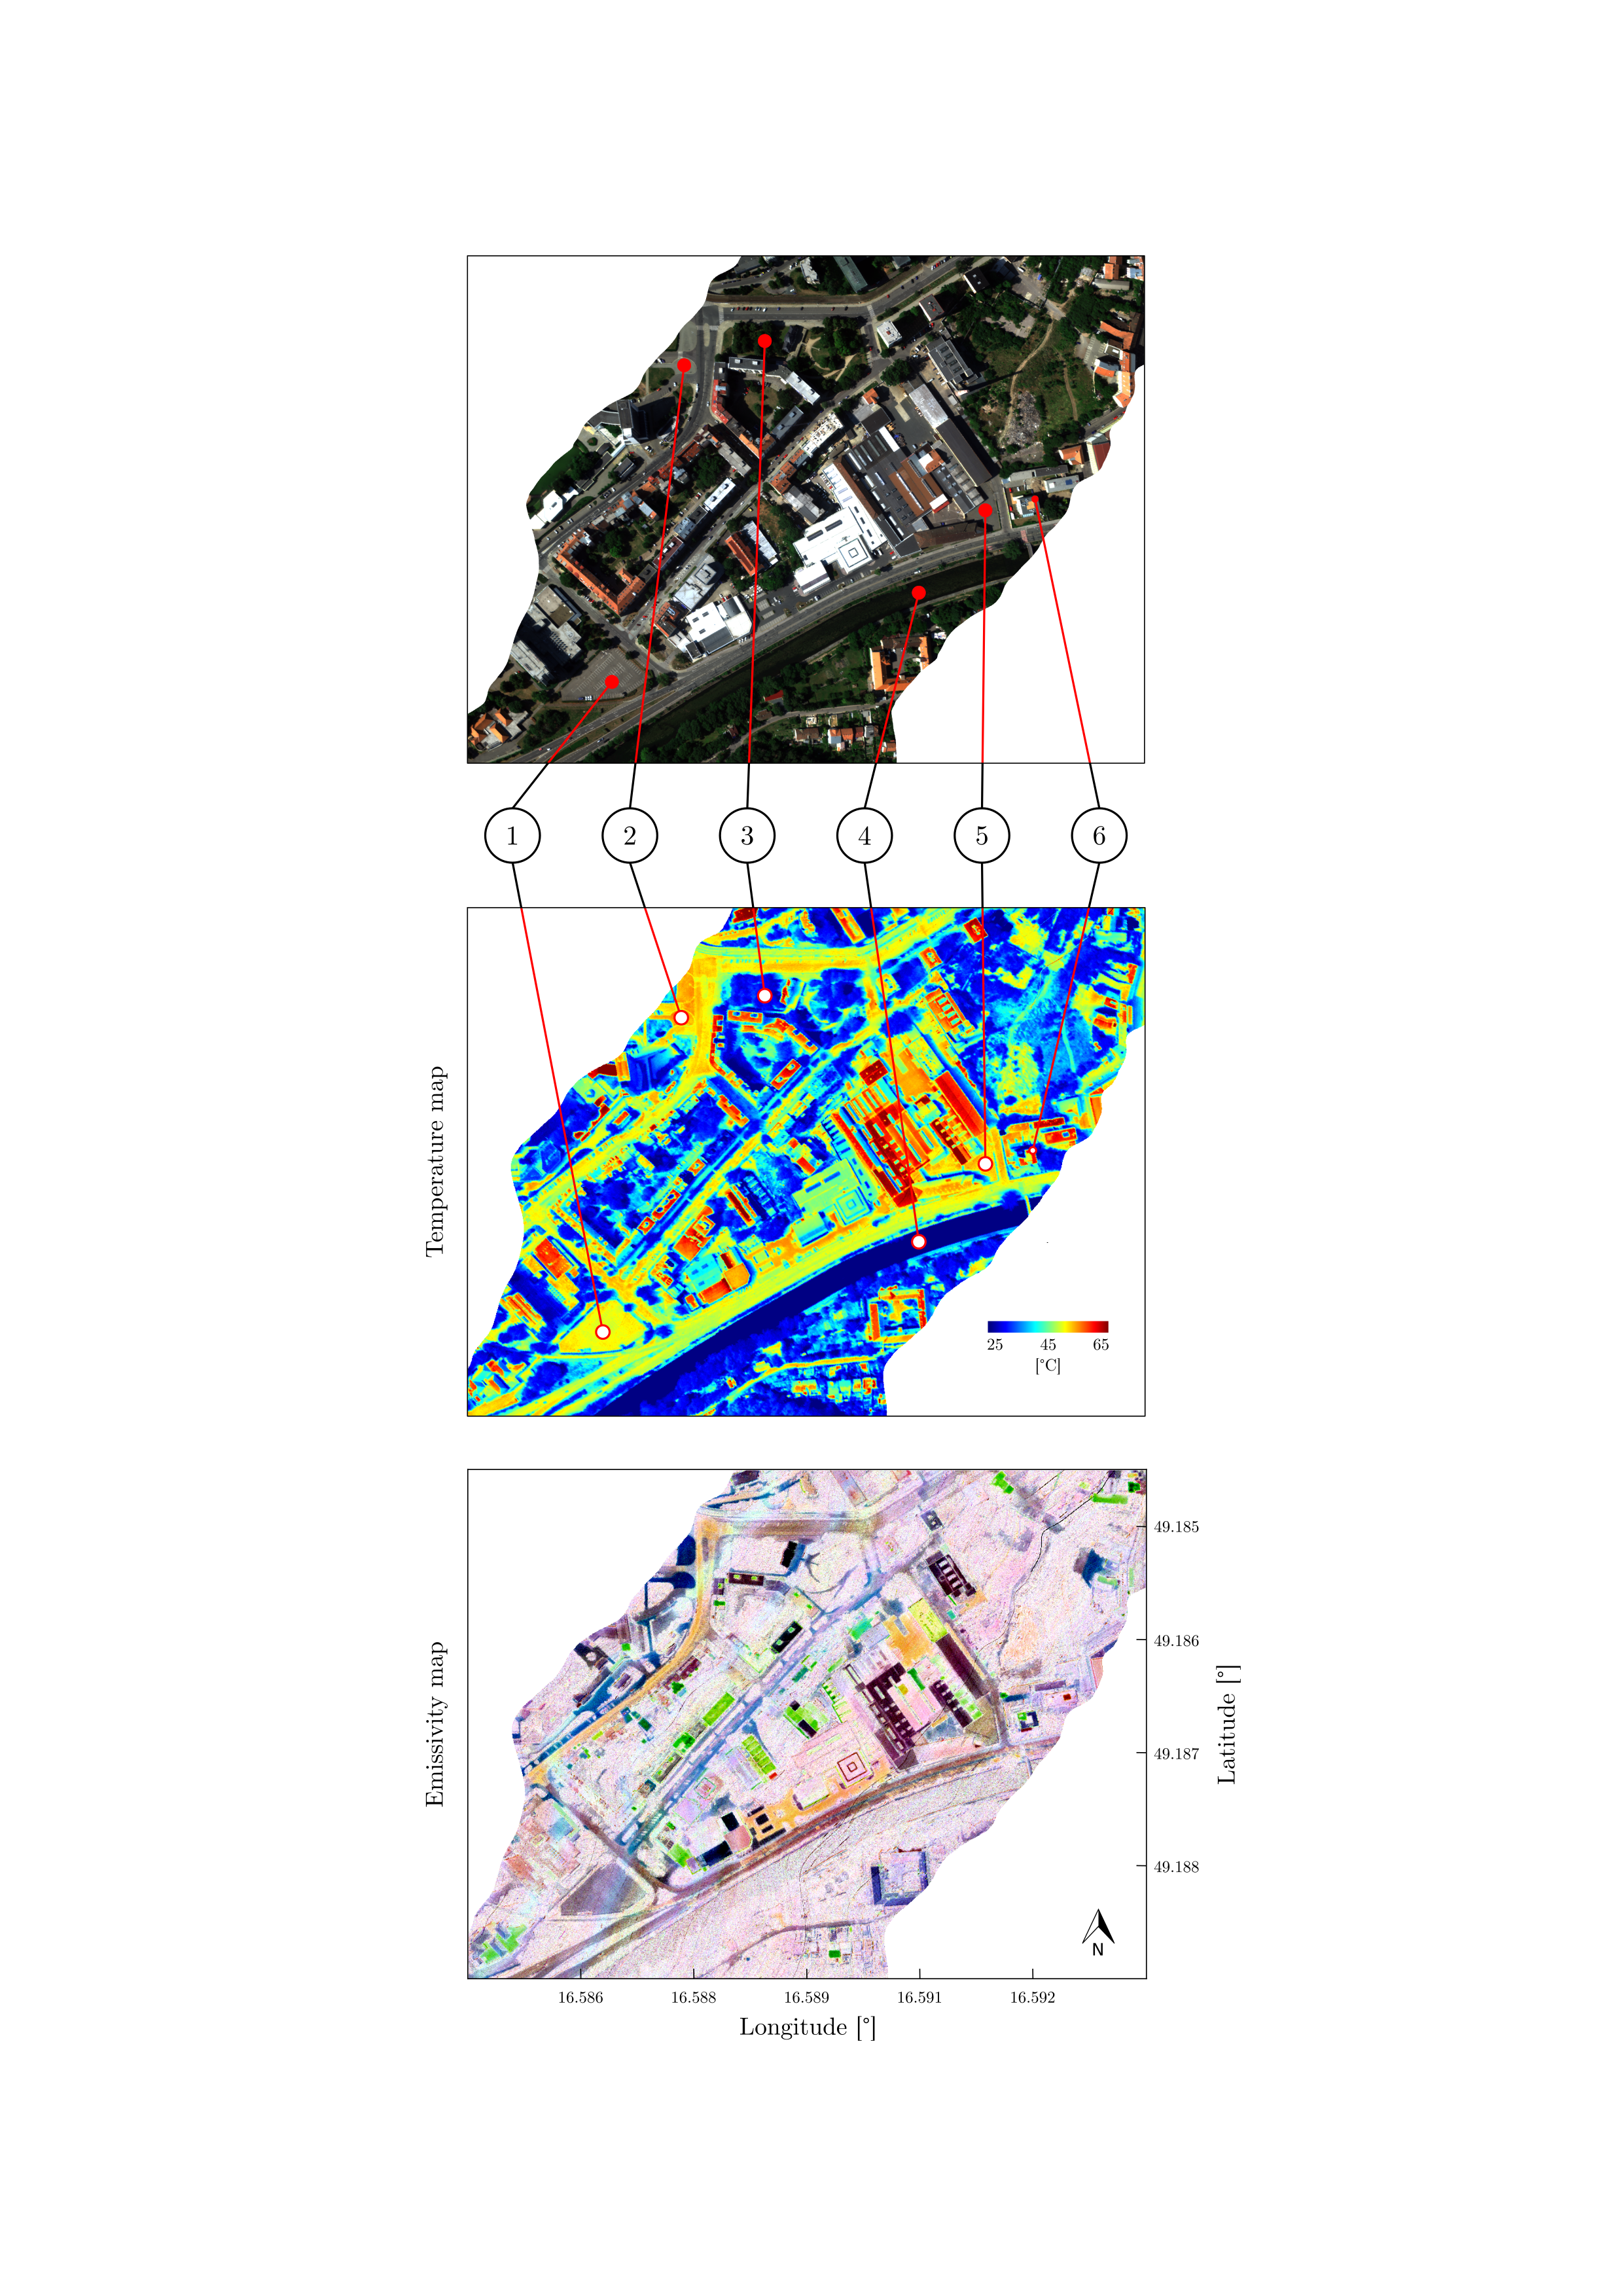
\includegraphics[scale=0.88]{pics/Chapter_04/Brno.pdf}
\vspace{2 em}
\caption{
Part of flight line over Brno city. Image data were acquired on 4.7.2015. The top image displays RGB composition for visualisation of the studied area. The middle image depicts temperature map obtained from OSTES algorithm applied on image data from TASI sensor. The bottom image is false color emissivity map obtained from OSTES algorithm (red - band 10, green - band 15, blue - band 20). On the top and middle images are shown spots on which were performed \textit{in-situ} emissivity measurements.}
\label{fig:Bajkal}
\end{figure*}

\begin{figure*}[!t]
\centering
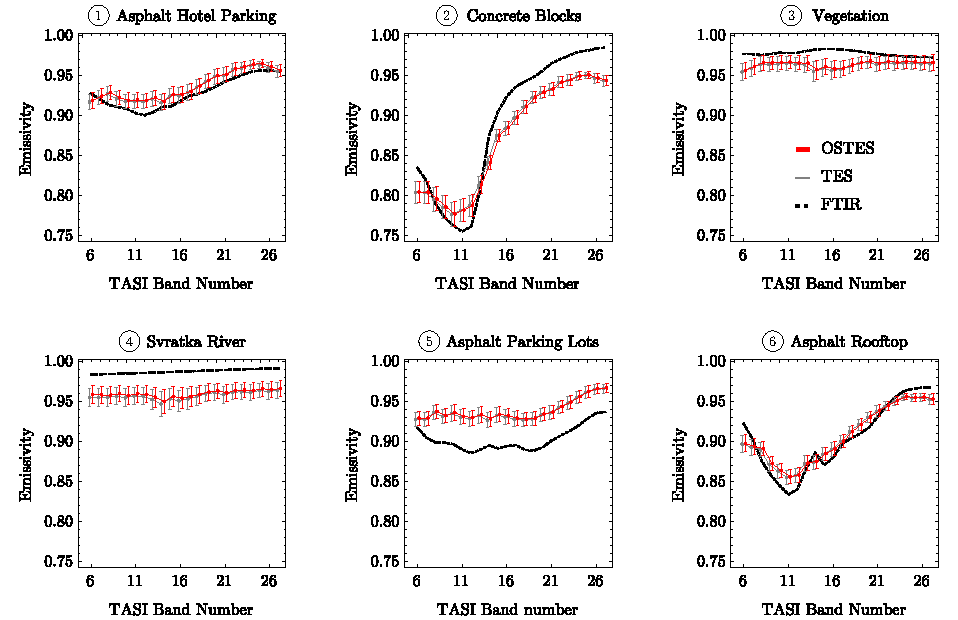
\includegraphics[width=0.95\linewidth]{pics/Chapter_04/Brno-Emissivity-Comparison.pdf}
\vspace{1.5 em}
\caption{Emissivity of Caspian Sea in different seasons obtained from ASTER standard product AST\_05, OSTES retrieval, and emissivity recomputation according to the temperature from AST\_08 and land-leaving and downwelling radiance from AST\_09T. Emissivities were extracted from area of size $40 \times 40$ pixels over pure and cloudless waterbody. Error bars display standard deviation.}
\label{fig:BrnoEmissivityComparison}
\end{figure*}